% ******************************************************************	********************************************
%
% **************************************************************************************************************
\documentclass[ twoside,openright,titlepage,numbers=noenddot,%
								toc=bibliography,toc=listof,%
                footinclude=false,headinclude=false,cleardoublepage=empty,%
								BCOR=5mm,paper=a4,fontsize=11pt,%DIV=14,%
                ngerman%
                ]{scrreprt}

%***************************************************************************************************************
% Note: Make all your adjustments in here
%***************************************************************************************************************
% ****************************************************************************************************
% htwsaar-i-mst-config.tex 
% ****************************************************************************************************  
\RequirePackage[utf8]{inputenc}				
 \DeclareUnicodeCharacter{00A0}{~}								
\RequirePackage[T1]{fontenc} 
								
% ****************************************************************************************************
% 1. Personal data and user ad-hoc commands
% ****************************************************************************************************
\newcommand{\myTitle}{Cloud-Native Architekturen}
\newcommand{\myDegree}{Bachelor of Science (B.\,Sc.)\xspace}
%\newcommand{\myDegree}{Master of Science (M.\,Sc.)\xspace}
\newcommand{\myDegreeType}{Bachelor\xspace}
%\newcommand{\myDegreeType}{Master\xspace}
\newcommand{\myDegreeCourse}{Praktische Informatik}
%\newcommand{\myDegreeCourse}{Kommunikationsinformatik}
\newcommand{\myName}{Tristan Gläs und Carolin Becker\xspace}
\newcommand{\myUni}{Hochschule für Technik und Wirtschaft des Saarlandes\xspace}
\newcommand{\myCompany}{SoftwareCenter Musterhausen\xspace}
\newcommand{\myFirstProf}{Prof. Dr. Markus Esch\xspace}
%\newcommand{\mySecondProf}{Prof. Dr. Thomas Kretschmer\xspace}
\newcommand{\myLocation}{Saarbrücken\xspace}
\newcommand{\myTime}{22.~März~2021\xspace}
\newcommand{\currentVersion}{Version 2.1\xspace} % TODO: ggf. über git Versionsinformationen automatisch bereitstellen und verwenden

% ********************************************************************
% Setup, finetuning, and useful commands
% ********************************************************************
\newcounter{dummy} % necessary for correct hyperlinks (to index, bib, etc.)
% ****************************************************************************************************


% ****************************************************************************************************
% 2. Loading some handy packages
% ****************************************************************************************************
% ******************************************************************** 
% Packages with options that might require adjustments
% ******************************************************************** 
\PassOptionsToPackage{ngerman}{babel}   % change this to your language(s)
 \RequirePackage{babel}					
 \RequirePackage{csquotes}
	
\PassOptionsToPackage{language=auto,style=numeric-comp,backend=bibtex8,bibencoding=ascii,maxbibnames=50}{biblatex}
 \RequirePackage{biblatex}	
 \bibliography{Bibliography}			

\PassOptionsToPackage{fleqn}{amsmath}		% math environments and more by the AMS 
 \RequirePackage{amsmath}

% ******************************************************************** 
% Setting up the page and margins
% ******************************************************************** 
\usepackage{geometry}
 \geometry{a4paper,left=25mm,right=35mm,top=25mm,bottom=30mm}
% DIESE WERTE SIND NICHT ZU VERÄNDERN -- DO NOT CHANGE THESE VALUES

% ******************************************************************** 
% General useful packages
% ******************************************************************** 
%\usepackage[automark]{scrpage2}
\PassOptionsToPackage{dvipsnames}{xcolor}
	\RequirePackage{xcolor} % [dvipsnames]  
	\definecolor{ingwi}{cmyk}{.9,0,0,0}
\usepackage{textcomp} % fix warning with missing font shapes
\usepackage{scrhack} % fix warnings when using KOMA with listings package          
\usepackage{xspace} % to get the spacing after macros right  
\usepackage{mparhack} % get marginpar right
%\usepackage{fixltx2e} % fixes some LaTeX stuff <-- ist seit 2015 nicht mehr notwendig
\PassOptionsToPackage{printonlyused}{acronym}
	\usepackage{acronym} % nice macros for handling all acronyms in the thesis
%\renewcommand{\bflabel}[1]{{#1}\hfill} % fix the list of acronyms
\usepackage{booktabs}
\usepackage{multirow}
\usepackage[shadow]{todonotes} %Settings for ToDoNotes
% Eigene Shortcuts fuer laengere Befehle
	\newcommand{\todox}[1]{\todo[inline, size=\small]{#1}}
	%Nummerierte Anmerkungen
	\newcounter{todocounter}
	\renewcommand{\todox}[2][]{\stepcounter{todocounter}\todo[inline, size=\small,caption={\thetodocounter: #2}, #1]{\renewcommand{\baselinestretch}{0.5}\selectfont\thetodocounter: #2\par}}
\usepackage{blindtext}
%\usepackage{footmisc}
% ****************************************************************************************************


% ****************************************************************************************************
% 3. Setup floats: tables, (sub)figures, and captions
% ****************************************************************************************************
\usepackage{tabularx} % better tables
	\setlength{\extrarowheight}{3pt} % increase table row height
%\newcommand{\myfloatalign}{\centering} % to be used with each float for alignment
\usepackage{caption}
\captionsetup{format=hang,font=small}
\usepackage{subfig}
\usepackage{wrapfig}
% ****************************************************************************************************


% ****************************************************************************************************
% 6. Setup code listings
% ****************************************************************************************************
\usepackage{listings} 
%\lstset{emph={trueIndex,root},emphstyle=\color{BlueViolet}}%\underbar} % for special keywords
\lstset{language=[LaTeX]Tex,%C++,
    keywordstyle=\color{RoyalBlue},%\bfseries,
    basicstyle=\small\ttfamily,
    %identifierstyle=\color{NavyBlue},
    commentstyle=\color{Green}\ttfamily,
    stringstyle=\rmfamily,
    numbers=none,%left,%
    numberstyle=\scriptsize,%\tiny
    stepnumber=5,
    numbersep=8pt,
    showstringspaces=false,
    breaklines=true,
    frameround=ftff,
    frame=single,
		texcl=true,
    belowcaptionskip=.75\baselineskip
    %frame=L
} 
%Styles für verschiedene Sprachen festlegen, z.B. Java
\lstdefinestyle{Java}{
belowcaptionskip=1\baselineskip,
  breaklines=true,
  xleftmargin=\parindent,
  language=Java,
	texcl=true,
  showstringspaces=false,
  basicstyle=\footnotesize\ttfamily,
  keywordstyle=\bfseries\color{green!40!black},
  commentstyle=\itshape\color{purple!40!black},
  identifierstyle=\color{blue},
  stringstyle=\color{orange}}
% ****************************************************************************************************    		   


% ****************************************************************************************************
% 6. PDFLaTeX, hyperreferences and citation backreferences
% ****************************************************************************************************
% ********************************************************************
% Using PDFLaTeX
% ********************************************************************
\PassOptionsToPackage{pdftex,hyperfootnotes=false,pdfpagelabels}{hyperref}
	\usepackage{hyperref}  % backref linktocpage pagebackref
\pdfcompresslevel=9
\pdfadjustspacing=1 
\PassOptionsToPackage{pdftex}{graphicx}
	\usepackage{graphicx} 
    

% ********************************************************************
% Hyperreferences
% ********************************************************************
\hypersetup{%
    %draft,	% = no hyperlinking at all (useful in b/w printouts)
    pdfstartpage=1, pdfstartview=Fit,%
		colorlinks=true, linktocpage=true,
		%urlcolor=Black, linkcolor=Black, citecolor=Black, %pagecolor=Black,%
		%urlcolor=brown, linkcolor=RoyalBlue, citecolor=green, %pagecolor=RoyalBlue,%
    % uncomment the following line if you want to have black links (e.g., for printing)
    colorlinks=false, pdfborder={0 0 0},
    breaklinks=true, pdfpagemode=UseNone, pageanchor=true, pdfpagemode=UseOutlines,%
    plainpages=false, bookmarksnumbered, bookmarksopen=true, bookmarksopenlevel=1,%
    hypertexnames=true, pdfhighlight=/O,%nesting=true,%frenchlinks,%
    pdftitle={\myTitle},%
    pdfauthor={\textcopyright\ \myName, \myUni},%
    pdfsubject={},%
    pdfkeywords={},%
    pdfcreator={pdfLaTeX},%
    pdfproducer={LaTeX with hyperref}%
}   

% ********************************************************************
% Setup autoreferences
% ********************************************************************
% There are some issues regarding autorefnames
% http://www.ureader.de/msg/136221647.aspx
% http://www.tex.ac.uk/cgi-bin/texfaq2html?label=latexwords
% you have to redefine the makros for the 
% language you use, e.g., american, ngerman
% (as chosen when loading babel/AtBeginDocument)
% ********************************************************************
\makeatletter
\@ifpackageloaded{babel}%
    {%
       \addto\extrasamerican{%
					\renewcommand*{\figureautorefname}{Figure}%
					\renewcommand*{\tableautorefname}{Table}%
					\renewcommand*{\partautorefname}{Part}%
					\renewcommand*{\chapterautorefname}{Chapter}%
					\renewcommand*{\sectionautorefname}{Section}%
					\renewcommand*{\subsectionautorefname}{Section}%
					\renewcommand*{\subsubsectionautorefname}{Section}% 	
				}%
       \addto\extrasngerman{% 
					\renewcommand*{\chapterautorefname}{Kapitel}%
					\renewcommand*{\sectionautorefname}{Abschnitt}%
					\renewcommand*{\subsectionautorefname}{Abschnitt}%
					\renewcommand*{\subsubsectionautorefname}{Abschnitt}% 
					\renewcommand*{\paragraphautorefname}{Absatz}%
					\renewcommand*{\subparagraphautorefname}{Absatz}%
					\renewcommand*{\footnoteautorefname}{Fu\"snote}%
					\renewcommand*{\FancyVerbLineautorefname}{Zeile}%
					\renewcommand*{\theoremautorefname}{Theorem}%
					\renewcommand*{\appendixautorefname}{Anhang}%
					\renewcommand*{\equationautorefname}{Gleichung}%        
					\renewcommand*{\itemautorefname}{Punkt}%
				}%	
			% Fix to getting autorefs for subfigures right (thanks to Belinda Vogt for changing the definition)
			\providecommand{\subfigureautorefname}{\figureautorefname}%  			
    }{\relax}
\makeatother


% ****************************************************************************************************
% 6. Last calls before the bar closes
% ****************************************************************************************************
% ********************************************************************
% Development Stuff
% ********************************************************************
%\listfiles
\PassOptionsToPackage{l2tabu,orthodox,abort}{nag}
	\usepackage{nag}
%\PassOptionsToPackage{warning, all}{onlyamsmath}
%	\usepackage{onlyamsmath}


% ****************************************************************************************************
% 7. Further adjustments (experimental)
% ****************************************************************************************************
%\usepackage{tocbibind} %Allows us to add Bibliography to ToC
\usepackage{enumitem}
\setdescription{font=\normalfont\bfseries} %Changes the appearance of description items
\usepackage[activate={true,nocompatibility},final,tracking=true,kerning=true,spacing=true,factor=1100,stretch=10,shrink=10]{microtype}


% ********************************************************************
% Using different fonts
% ********************************************************************
%\usepackage{lmodern} % <-- no osf support :-(
%\usepackage[tt=false]{libertine} % [osf]
%\usepackage{luximono} 
\usepackage{mathpazo} 
%\usepackage[urw-garamond]{mathdesign} <-- no osf support :-(

\setkomafont{disposition}{\bfseries}
% ****************************************************************************************************

%********************************************************************
% Hyphenation
%*******************************************************
%\hyphenation{put special hyphenation here}

% ********************************************************************
% GO!GO!GO! MOVE IT!
%*******************************************************
\begin{document}
\frenchspacing
\raggedbottom
\selectlanguage{ngerman} % american ngerman
\pagenumbering{roman}
\pagestyle{plain}
%*******************************************************
% Frontmatter
%*******************************************************
%*******************************************************
% Titlepage
%*******************************************************
\begin{titlepage}\linespread{1.5}\selectfont

\includegraphics[width=\linewidth]{Graphics/htwsaar_Logo_inwi_head_VF_4C_crop}
  \begin{center}
    \large  
    \hfill
    \vfill
    \begingroup
      \Large\bfseries\myDegreeType-Thesis 
    \endgroup
		
		\bigskip
		
    zur Erlangung des akademischen Grades \\
    \myDegree \\ 
    an der \myUni \\
    im Studiengang \myDegreeCourse \\
    der Fakultät für Ingenieurwissenschaften \\ 
    
  \vfill
	
  \begingroup
    \Large\bfseries\myTitle 
  \endgroup
	
	\bigskip
	
  vorgelegt von \\
  \myName
	
  \vfill
	
  betreut und begutachtet von \\
  \myFirstProf \\
  \mySecondProf 
	
  \vfill
	
  \myLocation, \myTime                   

    \end{center}       
\end{titlepage}   
\cleardoublepage%*******************************************************
% Declaration
%*******************************************************
\pdfbookmark[0]{Selbständigkeitserklärung}{declaration}
\chapter*{Selbständigkeitserklärung}
%\thispagestyle{empty}

Ich versichere, dass ich die vorliegende Arbeit (bei einer Gruppenarbeit: den entsprechend gekennzeichneten
Anteil der Arbeit) selbständig verfasst und keine anderen als die angegebenen Quellen und
Hilfsmittel benutzt habe.

Ich erkläre hiermit weiterhin, dass die vorgelegte Arbeit zuvor weder von mir noch von einer anderen Person an dieser oder einer
anderen Hochschule eingereicht wurde.

Darüber hinaus ist mir bekannt, dass die Unrichtigkeit dieser Erklärung eine Benotung der 
Arbeit mit der Note \glqq nicht ausreichend\grqq zur Folge hat und einen Ausschluss von der Erbringung 
weiterer Prüfungsleistungen zur Folge haben kann.
\bigskip
 
\noindent\textit{\myLocation, \myTime}

\smallskip

\begin{flushright}
    \begin{tabular}{m{5cm}}
        \\ \hline
        \centering\myName \\
    \end{tabular}
\end{flushright}
%\cleardoublepage%*******************************************************
% Sperrvermerk
%*******************************************************
% Der Sperrvermerk kann entfernt werden, wenn die Arbeit z.B. nicht im 
% Zusammenarbeit mit einem Unternehmen angefertigt wurde oder kein
% Sperrvermerk verlangt wird.

\pdfbookmark[0]{Sperrvermerk}{sperrvermerk}
\chapter*{Sperrvermerk}
%\thispagestyle{empty}

Die vorliegende Arbeit mit dem Titel "`\myTitle"' enthält vertrauliche Daten des Unternehmens \myCompany.

Die Arbeit darf nur dem Erst- und Zweitgutachter sowie befugten Mitgliedern des Prüfungsausschusses zugänglich gemacht werden. 
Eine Veröffentlichung und Vervielfältigung der Arbeit ist -- auch in Auszügen -- nicht gestattet.

Eine Einsichtnahme der Arbeit durch Unbefugte bedarf einer ausdrücklichen Genehmigung des Verfassers und des Unternehmens \myCompany.
 % <-- sollte in der Regel nicht notwendig sein und mit Betreuer/Unternehmen abgeklärt werden
\cleardoublepage%*******************************************************
% Abstract
%*******************************************************
\pdfbookmark[0]{Zusammenfassung}{Zusammenfassung}
\chapter*{Zusammenfassung}
Kurze Zusammenfassung des Inhaltes in deutscher Sprache, der Umfang beträgt zwischen einer halben und einer ganzen DIN A4-Seite.

Orientieren Sie sich bei der Aufteilung bzw. dem Inhalt Ihrer Zusammenfassung an Kent Becks Artikel: \url{http://plg.uwaterloo.ca/~migod/research/beckOOPSLA.html}.
\cleardoublepage%*******************************************************
% Acknowledgments
%*******************************************************
\pdfbookmark[0]{Danksagung}{acknowledgments}

% Beispiel für ein sinnvolles Zitat 
\begin{flushright}{\slshape    
    We have seen that computer programming is an art, \\ 
    because it applies accumulated knowledge to the world, \\ 
    because it requires skill and ingenuity, and especially \\
    because it produces objects of beauty.} \\ \medskip
    --- Donald E. Knuth \cite{knuth:1974}
\end{flushright}

\bigskip

\begingroup
	\let\clearpage\relax
	\let\cleardoublepage\relax
	\let\cleardoublepage\relax
	\chapter*{Danksagung}
	Hier können Sie Personen danken, die zum Erfolg der Arbeit beigetragen haben, beispielsweise Ihren Betreuern in der Firma, Ihren Professoren/Dozenten an der htw saar, Freunden, Familie usw.




\endgroup


\cleardoublepage%*******************************************************
% Table of Contents
%*******************************************************
\setcounter{tocdepth}{2} % <-- 2 includes up to subsections in the ToC
\setcounter{secnumdepth}{3} % <-- 3 numbers up to subsubsections

\pdfbookmark[0]{\contentsname}{toc}
\tableofcontents 

% Die weiteren Verzeichnisse folgen am Ende des Dokuments 

                  


%*******************************************************
% Mainmatter
%*******************************************************
\cleardoublepage
\pagenumbering{arabic}
\pagestyle{headings}
%\pagestyle{scrheadings}
\cleardoublepage%=========================================
% 	   Einleitung     		 =
%=========================================
\chapter{Einleitung}

\begin{description}
	\item [TeXnicCenter] Umfangreiche Entwicklungsumgebung mit Projektorganisation und Autovervollständigung
	\item [TeXLipse] Eclipse-Plugin, das alle Vorteile der Eclipseumgebung mit LaTeX verbindet
	\item [TeXmaker] Einfacher LaTeX-Editor mit Pdf-Direktvorschau
\end{description}	 	% Diese Einbindungen werden natürlich entfernt, wenn es an die richtige
\cleardoublepage%*****************************************
\chapter{Beispiele}\label{ch:examples}
%*****************************************

%************************************************
%*  Abkürzungen *********************************
%************************************************

\section{Abkürzungen}

Um Abkürzungen zu verwenden, muss über \lstinline|\usepackage{acronym}| das benötigte Package geladen werden. Danach kann man lange Begriffe ganz bequem abkürzen:

So muss man nicht ständig \ac{WLAN} ausschreiben, auch \ac{TCP} lässt sich abkürzen. Würde man im Text \acs{WLAN} oft verwenden, kann man sie, wie hier, nur als
Abkürzung anzeigen lassen - oder bei Bedarf die Erklärung mitliefern (\acf{WLAN}). Weiteres Beispiel könnte die \ac{GoF} sein.

Weitere Informationen sind im \href{http://www.ctan.org/tex-archive/macros/latex/contrib/acronym}{Acronym-Manual} zu finden.
%*********************************************
%*	Biblatex-Beispiel
%*********************************************
\section{Beispiel für BibLaTeX}

BibLaTeX ist ein Package, das einem die Arbeit mit Zitaten bzw. Quellenangaben erleichtern kann. Mit JabRef (\autoref{sec:Werkzeuge}) ist es möglich
\textit{*.bib}-Dateien zu erstellen, in denen alle Angaben zu Autor, Buchtitel, Erscheinungsdatum usw. hinterlegt werden, welche zum passenden Zeitpunkt
abgerufen werden können. Das Literaturverzeichnis wird mittels \lstinline{\printbibliography} ausgegeben.

Im Allgemeinen wird im Literaturverzeichnis auch nur jene Literatur aufgenommen, die auch in der \textit{*.tex}-Datei referenziert wird. Danach ist es wichtig
nicht nur mit \textit{Pdf\-LaTeX}, sondern auch mit \textit{BibLaTeX} zu kompilieren, damit die zitierten Einträge in die verschiedenen Hilfsdateien aufgenommen
werden können. %Hinweis: Pdf\-LaTeX teilt LaTeX mit, dass nur zwischen Pdf und LaTeX getrennt werden darf


\subsection*{Einige Zitate}
In diesem Satz könnten wir auf \cite{knuth:1976} verweisen, ebenso auf das wichtige Werk \cite{dueck:trio}. Wenn uns das nicht genug ist, sollten wir das anmerken,
was in \cite{sommerville:1992} geschrieben wurde. Im Zweifelsfall verweisen wir auf eine einzelne Seite, wie in \cite[112]{bentley:1999} zu finden. 

Üblicherweise wird auch der Name des Autors bzw. der Autoren genannt, also beispielsweise bei einem Verweis auf \citeauthor{knuth:1976} \cite{knuth:1976} oder 
auch bei mehreren Autoren \citeauthor{cormen:2001} \cite{cormen:2001}. LaTeX stellt Mechanismen zur Verfügung, auch dies automatisiert zu erledigen.





\section{Referenzierungen}
Mit Referenzierungen kann ich ganz bequem auf Textpassagen, Kapitel, Sections oder Abbildungen im weiteren Text verweisen.
Dies ist ein Verweis auf \autoref{subsec:Beispieltext}, der sich auf \autoref{subsec:Beispieltext} befindet.

Auch ein Verweis auf \autoref{tab:beispieltabelle1} auf Seite~\pageref{tab:beispieltabelle1} ist möglich.

Man sollte beachten, dass man sein Dokument, wenn es Referenzierungen enthält, mehrmals kompiliert, da sonst manche
Verweise nicht aufgelöst werden können.


\subsection{Beispieltext}\label{subsec:Beispieltext}
\blindtext

\section{Dateien einbinden}

Damit man nicht alle Einstellungen, Optionen, Packages und Texte, Abbildungen etc. in einer Datei unterbringen muss, werden
zwei Befehle bereitgestellt, um externe \textit{*.tex}-Dateien einzubinden: \lstinline|\include{PFAD}| und \lstinline|\input{PFAD}|.
Mit dem erstem Befehl wird eine neue Seite angelegt, danach kommen die Inhalte aus der angegebenen Datei; mit dem zweiten
Befehl wird keine neue Seite angelegt -- der Inhalt der angegebenen Datei wird direkt an die betroffene Stelle eingefügt.

\textbf{Wichtig:} Der \textit{Pfad} wird sinnigerweise \textit{relativ} angegeben, wobei als Stammverzeichnis jenes Verzeichnis
angesehen wird, in dem die \textit{*.tex}-Datei mit der \textit{Document}-Umgebung abgelegt ist (in diesem Fall ist es 
\textit{htwsaar-i-mst-config.tex}).
%************************
%*		Tabellen 		*
%************************

\section{Tabellen}
\label{sec:Tabellen}

\subsection{Einfache Tabelle}
In LaTeX lassen sich Tabellen unterschiedlicher Ausprägung einfach erzeugen. Das allgemeine Format einer Tabelle sieht aus wie folgt:

\begin{lstlisting}[caption={Allgemeines Format}]
\begin{table}
	\caption{BESCHRIFTUNG}
	\begin{tabular}{FORMATIERUNG}
		TABELLENINHALT
	\end{tabular}
\end{table}
\end{lstlisting}

Eine Beispieltabelle (Tabelle \ref{tab:beispieltabelle1}) könnte also so aussehen:

\begin{lstlisting}[caption={Tabelle \ref{tab:beispieltabelle1}}]
\begin{table}
	\caption{Beispiel 1}
	\begin{tabular}{lrcr}
		\toprule
		\textbf{Name} & \textbf{Vorname} & \textbf{Matrikelnummer} & \textbf{Lieblingsspeise}\\
		\midrule
		Jackson & Michael & 123456 & Erdbeereis \\
		Springsteen & Bruce & 234567 & Schwedisches Lakritz \\
		Bach & Anna, Magdalena & 3456789 & Frankfurter Kranz \\
		Schumann & Clara & 4567890 & Bisquitt\"ortchen \\
		\bottomrule
	\end{tabular}
	\label{tab:beispieltabelle1}
\end{table}
\end{lstlisting}

Mit \lstinline|\caption{Beispiel 1}| bekommt unsere Tabelle eine Beschriftung am Tabellenkopf. \lstinline{l|r|c|r} legt die Textausrichtung der einzelnen Spalten fest: \lstinline|l| bedeutet linksausgerichtet, \lstinline|r| rechtsausgerichtet und \lstinline|c| zentriert. Durch \lstinline{|} werden Spaltenlinien gezogen. \lstinline|\toprule|, \lstinline|\midrule| und \lstinline|\bottomrule| erzeugen Kopf-, Mittel- und Abschlusslinie in der Tabelle. Als Spaltentrenner wird das \lstinline{&} genutzt, Zeilentrenner ist der doppelte Backslash (\lstinline|\\|). Am Ende kann die Tabelle auch mit einem Label versehen werden (\lstinline|\label{tab:beispieltabelle1}|), über welches diese referenziert wird.

%\begin{center}
\begin{table}[b]
	
	\caption{Beispiel 1}
	\begin{tabular}{lrcr}
		\toprule
		\textbf{Name} & \textbf{Vorname} & \textbf{Matrikelnummer} & \textbf{Lieblingsspeise}\\
		\midrule
		Jackson & Michael & 123456 & Erdbeereis \\
		Springsteen & Bruce & 234567 & Schwedisches Lakritz \\
		Bach & Anna, Magdalena & 3456789 & Frankfurter Kranz \\
		Schumann & Clara & 4567890 & Bisquittörtchen \\
		\bottomrule
	\end{tabular}
	\label{tab:beispieltabelle1}
\end{table}
%\end{center}

\subsection{Erweiterte Tabellenbefehle}
Um Tabellen in LaTeX flexibler zu gestalten gibt es weitere Befehle bzw. zusätzliche Pakete, die einem das Leben leichter machen (Tabelle \ref{tab:beispieltabelle2}). Hierzu ein weiteres Beispiel:

\begin{lstlisting}[caption={Tabelle \ref{tab:beispieltabelle2}}]
\begin{table}
	\centering
	\caption{Beispiel 2}
	\begin{tabular}{lll}
		\hline
		Author & Title & Year \\
		\hline
		\hline
		\multirow{3}{*}{Stanislav Lem} & Solaris & 1961 \\
 			& Roboterm\"archen & 1967 \\
 			& Der futurologische Kongress & 1971 \\
		\hline
		\multirow{3}{*}{Isaac Asimov} & Ich, der Robot & 1952 \\
 			& Der Tausendjahresplan & 1966 \\
 			& Doctor Schapirows Gehirn & 1988 \\
		\hline
	\end{tabular}
\label{tab:beispieltabelle2}
\end{table}
\end{lstlisting}

Mit \lstinline|\centering| wird die Tabelle zentriert ausgerichtet, analoge Befehle für rechts- bzw. linksausrichtung sind z.B. \lstinline|\raggedleft| und \lstinline|\raggedright|. \\

Eine weitere Form der Tabellen ist das Package \textit{tabularx}, das variable Spaltenbreiten unterstützt, und \textit{booktabs}, welches mit horizontalen Linien besser arbeiten kann.
\begin{table}
	\centering
	\caption{So sollte man es nicht machen! Beispiel für einen schlechten Tabellenstil}
	\begin{tabular}{|l|l|l|}
		\hline
		Author & Title & Year \\
		\hline
		\hline
		\multirow{3}{*}{Stanislav Lem} & Solaris & 1961 \\
 			& Robotermärchen & 1967 \\
 			& Der futurologische Kongress & 1971 \\
		\hline
		\multirow{3}{*}{Isaac Asimov} & Ich, der Robot & 1952 \\
 			& Der Tausendjahresplan & 1966 \\
 			& Doctor Schapirows Gehirn & 1988 \\
		\hline
	\end{tabular}
\label{tab:beispieltabelle2}
\end{table}
\section{Abbildungen}
%=============================

\textit{LaTeX} unterstützt generell die Formate \textit{*.jpeg}, \textit{*.png} und \textit{*.pdf}.
Handelt es sich z.B. um Strichgrafiken oder skalierbare Farbflächen, sollte \textit{*.pdf} die erste Wahl sein,
da sich in diesem Format Vektorgrafiken ohne Qualitätsverlust darstellen bzw. skalieren lassen.

\begin{figure}[bth] 
  \centering
  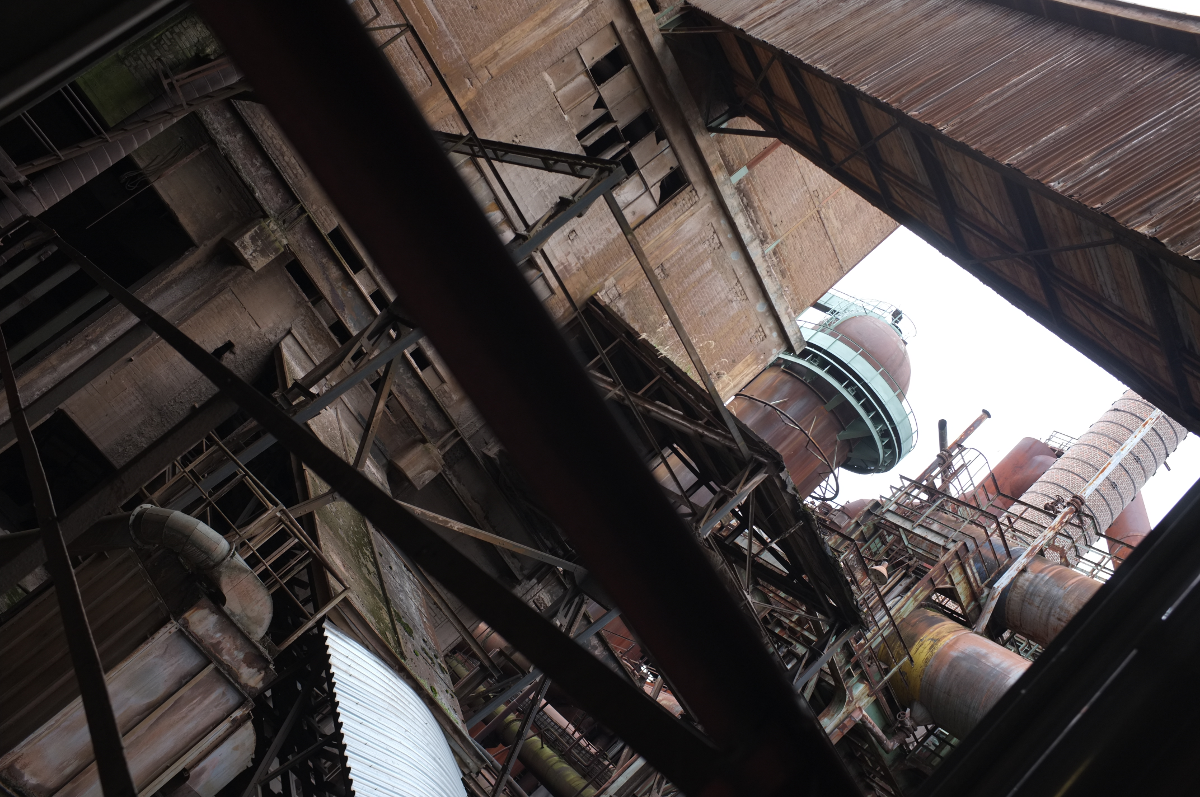
\includegraphics[width=0.7\textwidth]{Examples/example_5.png}
  \caption{Erstes Bild, Völklinger Hütte}
  \label{fig:Huette}
\end{figure}


\subsection{Wrapfigure}
Abbildung~\ref{fig:Huette} ist zwar ganz nett anzusehen, aber vielleicht sähe es eleganter aus, wenn die Abbildung 
von unserem Textabschnitt umflossen werden würde. Diese Art von Abbildungen sollte jedoch sparsam und mit großer Sorgfalt eingesetzt werden, da es zu unschönen Darstellungen kommen kann.
\blindtext
\begin{wrapfigure}{l}{0.4\textwidth}
  \centering
  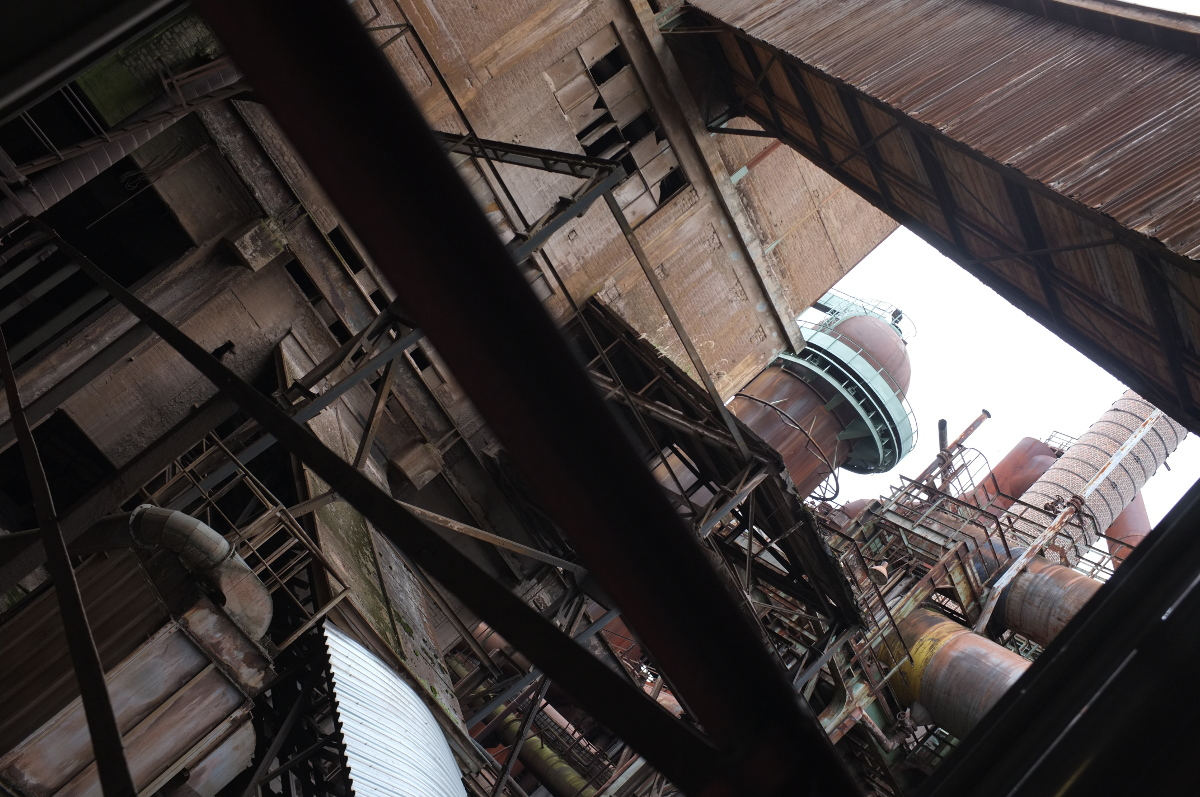
\includegraphics[width=0.4\textwidth]{Examples/example_5.jpg}
  \caption{Völklinger Hütte, *.jpg}
  \label{fig:Huette2}
\end{wrapfigure}
\blindtext


\subsection{Subfigures}
Es ist ebenso möglich, mehrere Abbildungen nebeneinander zu setzen, wie in Abbildung~\ref{fig:Beide} zu sehen ist. Eine separate Referenzierung ist auch möglich: Abbildung~\ref{subfig:abbone}.
\begin{figure}[bth]
  \subfloat[Erstes ...]{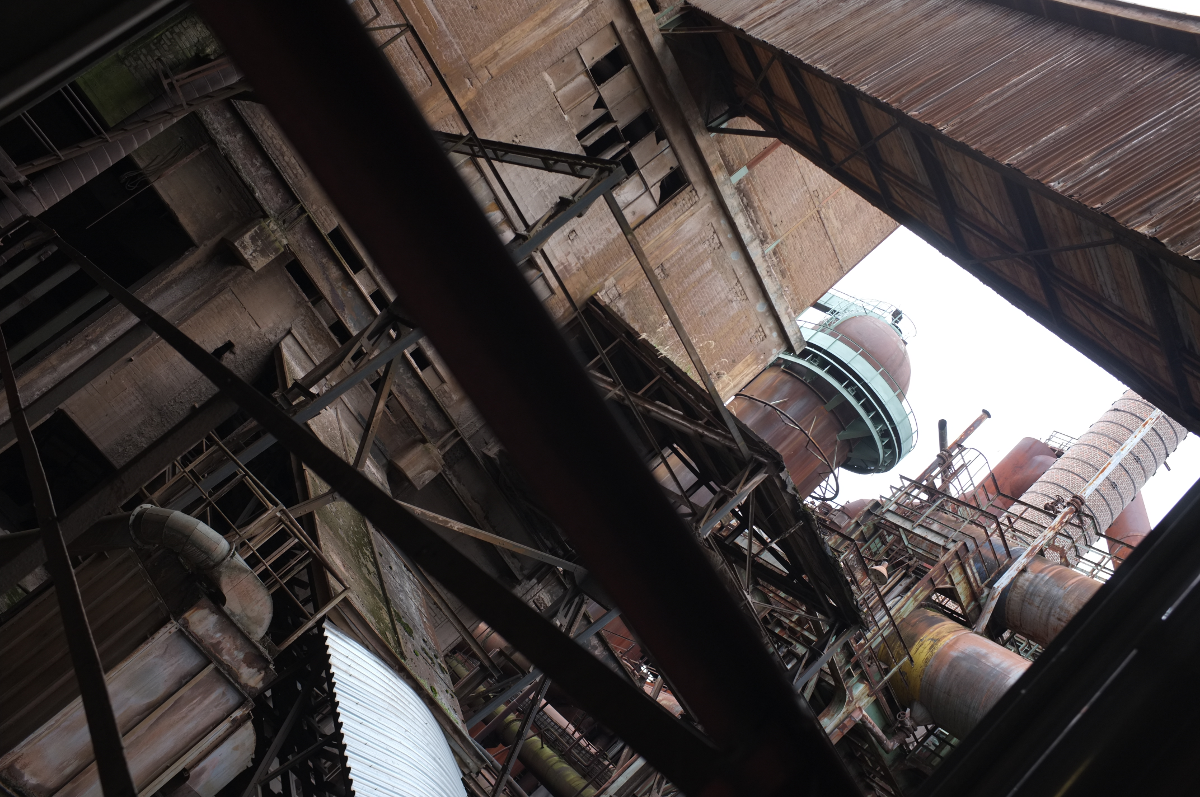
\includegraphics[width=0.49\textwidth]{Examples/example_5.png}\label{subfig:abbone}}\hfill
  \subfloat[... und zweites Bild]{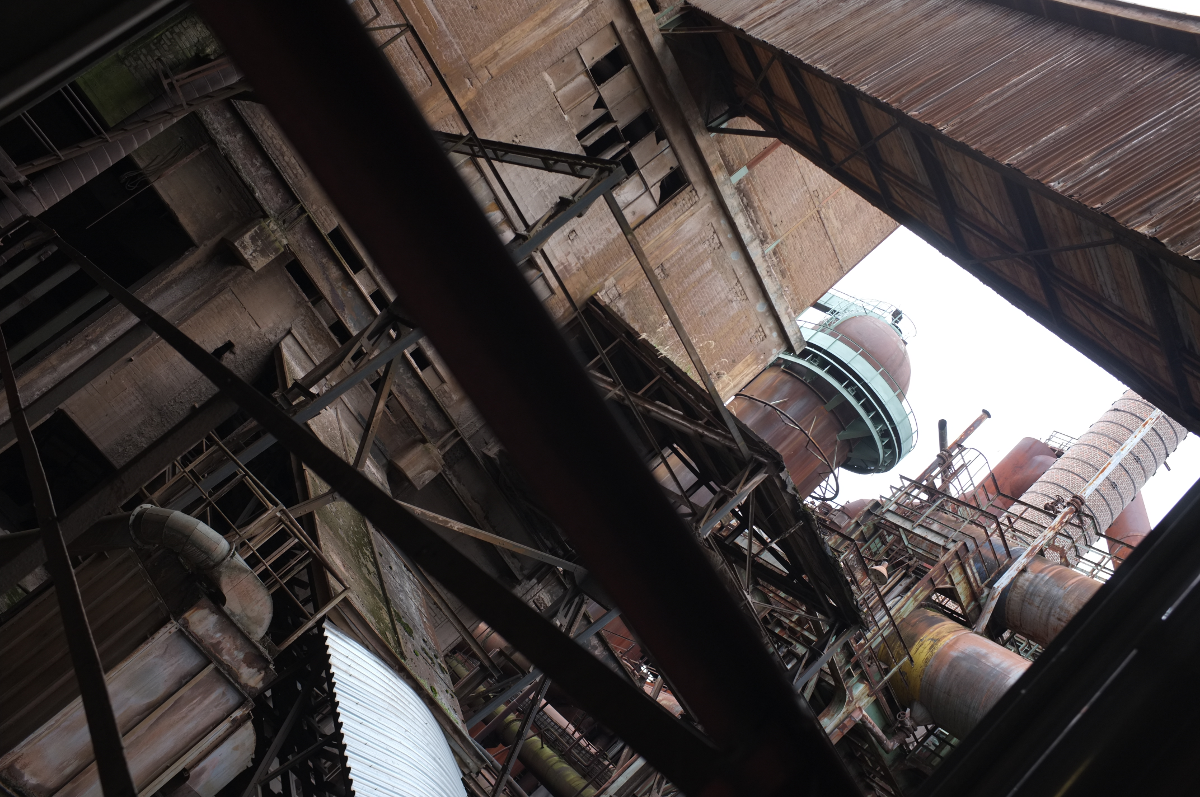
\includegraphics[width=0.49\textwidth]{Examples/example_5.png}\label{subfig:abbtwo}}
  \caption{Mehrere Abbildungen nebeneinander}
  \label{fig:Beide}
\end{figure}


\subsection{Qualitätsunterschiede}
\begin{figure}[p]
	\centering
  \subfloat[\textit{PDF}-Format]{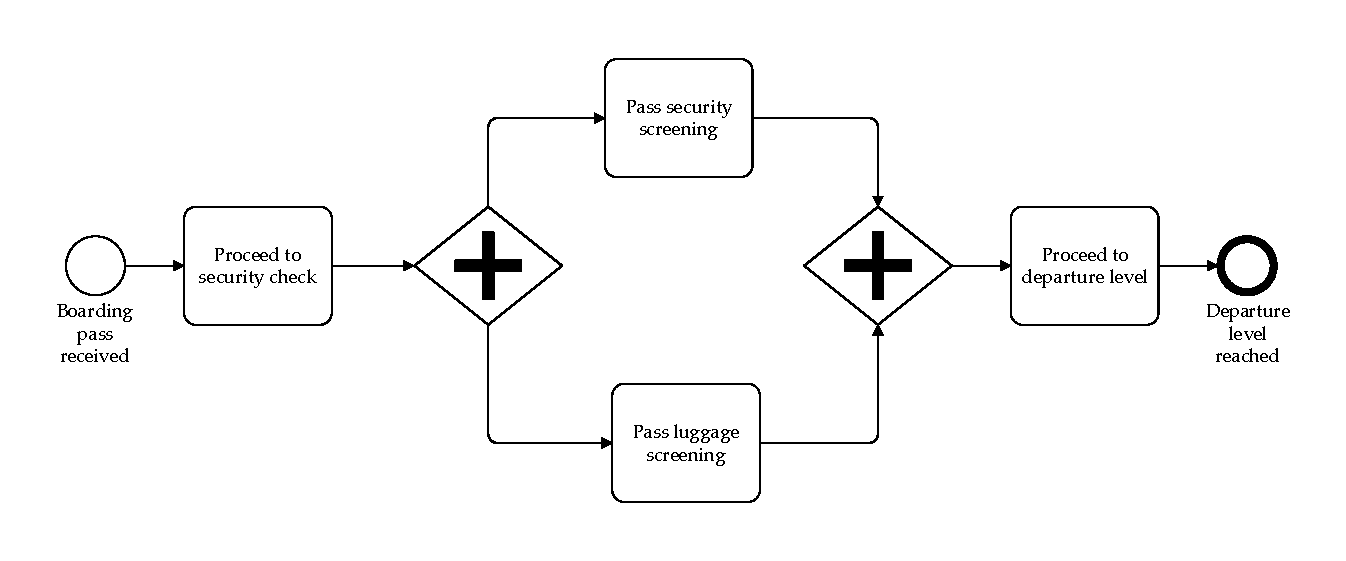
\includegraphics[width=0.65\textwidth]{Examples/bpmn.pdf}} \\
  \subfloat[\textit{JPG}-Format]{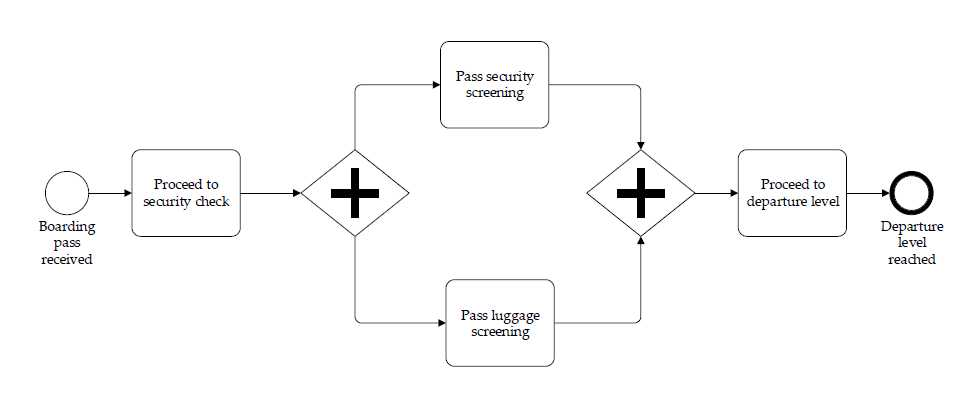
\includegraphics[width=0.65\textwidth]{Examples/bpmn.jpg}}
  \caption{Beide Formate im Vergleich}
  \label{fig:pdfvsjpg}
\end{figure}

\begin{figure}[p]
	\centering
  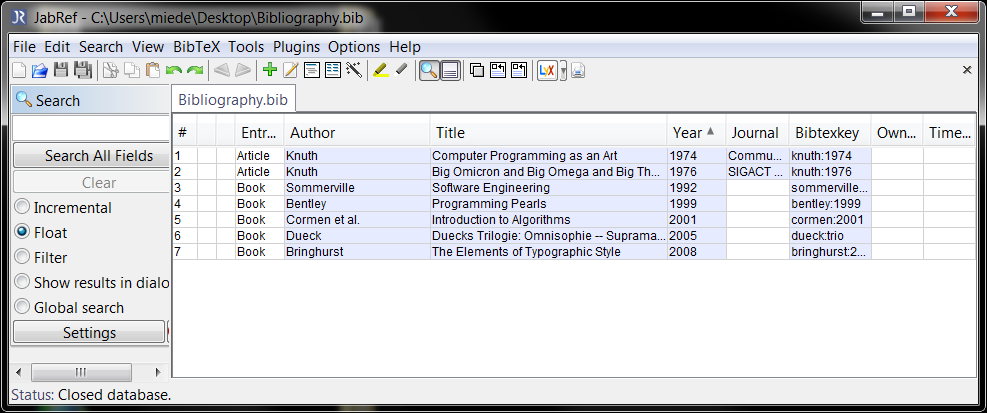
\includegraphics[width=0.65\textwidth]{Examples/jabref.png}
   \caption{\textit{PNG}-Format}
  \label{fig:pngvsjpg1}
\end{figure}

\begin{figure}[p]
	\centering
  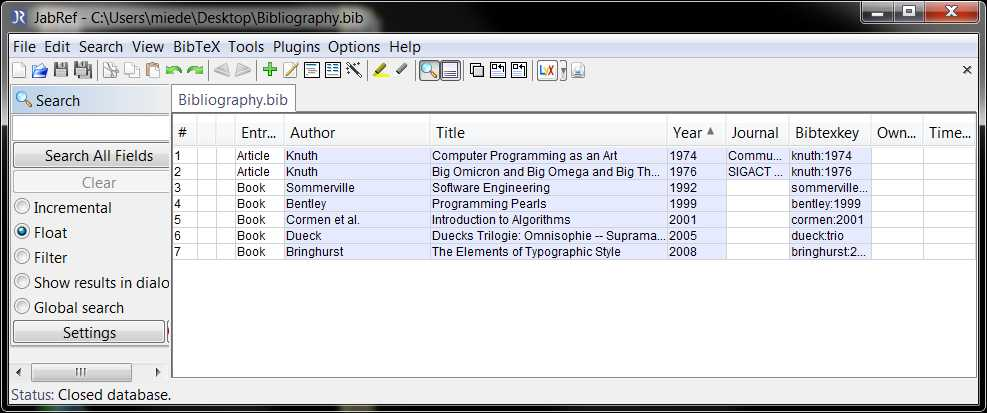
\includegraphics[width=0.65\textwidth]{Examples/jabref.jpg}
   \caption{\textit{JPG}-Format}
  \label{fig:pngvsjpg2}
\end{figure}

Leider haben die unterschiedlichen Grafikformate bedingt durch die unterschiedlichen Kompressionsverfahren einige Schwächen, insbesondere die Umwandlung in das \textit{JPG}-Format erzeugt unangenehme Artefakte im Bild. \autoref{fig:pdfvsjpg} zeigt die Unterschiede zwischen \textit{PDF-Format} und \textit{JPG-Format} im Vergleich. 

Wenn eine \textit{*.pdf}-Datei nicht infrage kommt, beispielsweise bei Screenshots, ist unbedingt das \textit{PNG-Format} vorzuziehen. 
Den Unterschied machen \autoref{fig:pngvsjpg1} und \autoref{fig:pngvsjpg2} deutlich.

\glqq Faustregeln\grqq im Umgang mit Abbildungen:
\begin{itemize}
	\item Diagramme bzw. alles, was Linien usw. enthält: \textit{PDF} (im Vektorformat).
	\item Screenshots bzw. alles, was größere gleichfarbige Flächen enthält: \textit{PNG}.
	\item Der Rest (in der Regel Fotos): \textit{JPEG}.
\end{itemize}





%*******************************
% 			Listings 		   *
%*******************************

\section{Quellcode einbinden}
Das Package \textit{lstlisting} ermöglicht es, Quellcode ansprechend in das Dokument einzubinden. Man kann Quellcode einzeilig einbinden 
mittels \lstinline{\lstinline|Quellcode|}. Dabei ist darauf zu achten, dass der Befehl einmal mit \{ \} und einmal mit | | aufgerufen werden kann, je nachdem, 
welche Zeichen im angegebenen Quelltext genutzt werden. 
Es ist auch möglich eine eigene Umgebung für Quelltext zu schaffen:

\begin{lstlisting}[caption=Erstes Listing,style=Java]
private Umgebung(int i, int k)
{
	System.out.println("Eine Funktion mit " + i + "und" + k ".");
}
\end{lstlisting}  

Wer Quelltext aus externen Dateien einbinden möchte, geht wie folgt vor:

\lstinputlisting
[caption={Externer Quellcode},style=Java]
{Examples/Code.java}

Wie genau der Quellcode formatiert und gefärbt ist, ist in \textit{htwsaar.i.mst.config.tex} hinterlegt, wobei fü verschiedene Sprachen auch eigene Styles angelegt werden
können (hier z.B. für Java).
\section{Mathematische Ausdrücke}
Mathematische Ausdrücke sind eine kleine Kunst für sich. Am allereinfachsten kann man eine Formel, wie \(a + b = c\) in den Fließtext einbinden, wobei LaTeX die Höhe der Ausdrücke der Zeile anpasst,
wie hier zu sehen \(\sum_{y=0}^{x} a\) . In einer Umgebung sieht das schon anders aus:
\begin{equation}
  \sum_{y=0}^{x} a
\end{equation}

Griechische Buchstaben:
\begin{equation}
	\alpha\beta\gamma\delta\epsilon\varepsilon\zeta\eta
	\theta\iota\kappa\lambda\mu\nu\xi\pi\varpi\rho\varrho
	\sigma\tau\upsilon\phi\varphi\chi\psi\omega
\end{equation}

Brüche:
\begin{equation}
	Ergebnis = \frac{a}{b}
\end{equation}

\begin{equation}
	\frac{\sin{\alpha}^2 + \cos{\alpha}^2}{1} = 1
\end{equation}

\begin{equation}
	\frac{-9x}{\frac{2y}{3z+2}}
\end{equation}

Text innerhalb von Formeln:
\begin{equation}
\sum_{y=1}^{n} y = \frac{n*(n+1)}{2}
\quad
\text{Gaußsche Summenformel}
\end{equation}

Hoch- bzw. Tiefstellungen:
\begin{equation}
	x_{i,j}^2
\end{equation}

\begin{equation}
	{x_{i,j}}^2
\end{equation}

\begin{equation}
	x_{n_0}
\end{equation}


Matrizen:
Matrizen werden innerhalb der mathematischen Umgebung als wiederum neue Umgebung eingebunden. Wie bei Tabellen auch werden Zeilen durch \lstinline{\\} und Spalten durch \lstinline{&} getrennt.

\begin{equation}
	\begin{pmatrix} 
		a&b\\
		c&d 
	\end{pmatrix}
\end{equation} 

\begin{equation}
	\begin{vmatrix} 
		a&b\\
		c&d 
	\end{vmatrix}
\end{equation} 

Fallunterscheidung:
\begin{equation}
	f(x) = 
	\begin{cases}
		0, &\text{falls } x < 0 \\
		1, &\text{falls } x \geq 0
	\end{cases}
\end{equation}




%############################################################
\clearpage\section{To-Do-Notes}
Um bei einer längeren Arbeit nicht den Überblick zu verlieren, an welcher Stelle es nötig ist
weiter zu arbeiten, bietet es sich an, kleine Notizen einzufügen. Das Package \textit{todonotes}
stellt eine elegante Lösung bereit, um differenziert und vielfarbig jene Abschnitte zu kennzeichnen,
die einer weiteren Bearbeitung bedürfen.

\subsection*{Beispiel für To-Do-Notes}
Dies hier ist ein Blindtext zum Testen von Textausgaben. Wer diesen Text liest, ist selbst
\todo{Plain todonotes.} schuld. Der Text gibt lediglich den Grauwert der Schrift an. Ist das wirklich so? Ist es
gleichgültig, ob ich schreibe: Dies ist ein Blindtext? oder Huardest gefburn? Kjift?
mitnichten! Ein Blindtext bietet mir wichtige Informationen. An ihm messe ich die Les-
barkeit einer Schrift, ihre Anmutung, \todo{Plain todonotes.}wie harmonisch die Figuren zueinander stehen
und prüfe, wie breit oder schmal sie läuft. Ein Blindtext sollte möglichst viele verschie-
dene Buchstaben enthalten und in der Originalsprache gesetzt sein. Er muss keinen
Sinn ergeben, sollte aber lesbar sein.\todo[nolist]{Todonote that is only shown in the margin and not in
the list of todos.}%
Fremdsprachige Texte wie Lorem ipsum dienen
nicht dem eigentlichen Zweck, da sie eine falsche Anmutung vermitteln. Dies hier ist
ein Blindtext zum Testen von Textausgaben. Wer diesen Text liest, ist selbst schuld. 

\todo[inline]{A very long todonote that certainly will fill more
than a single line in the list of todos. Just to make sure let's add
some more text \ldots}

Der Text gibt lediglich den Grauwert der Schrift an. Ist das wirklich so? Ist es gleichgültig,
ob ich schreibe: Dies ist ein Blindtext? oder Huardest gefburn? Kjift? mitnichten!
\todo[noline]{A note with no line back to the text.}
Ein Blindtext bietet mir wichtige Informationen. An ihm messe ich die Lesbarkeit einer
Schrift, ihre Anmutung, wie harmonisch die Figuren zueinander stehen und prüfe, wie
\todo[caption={A short entry in the list of todos}]{A very long
todonote that certainly will fill more than a single line in the
list of todos \ldots}
breit oder schmal sie läuft. Ein Blindtext sollte möglichst viele verschiedene Buchstaben
enthalten und in der Originalsprache gesetzt sein. Er muss keinen Sinn ergeben, sollte
aber lesbar sein. Fremdsprachige Texte wie Lorem ipsum dienen nicht dem eigentlichen Zweck, 
da sie eine falsche Anmutung vermitteln.
\missingfigure{A figure I have to make \ldots}

%Nummerierte ToDo-Notes
\todox{Erste Nummer...}
\todox{Zweite Nummer...}

%Alles To-Dos als Liste ausgegeben
Nachfolgend wird noch eine Liste aller To-Dos auf einer separaten 
Seite ausgegeben.
%\begingroup
	%\let\clearpage\relax
	%\let\cleardoublepage\relax
	\listoftodos
%\endgroup 


 		% Abschlussarbeit geht!
\cleardoublepage%=========================================
% 	   Grundlagen     		 =
%=========================================
\chapter{Grundlagen}

\section{\LaTeX\ installieren und einrichten}
\subsection{Unter Windows}

Als LaTeX-Distribution unter Windows steht \href{http://www.miktex.org/}{\textit{MikTeX}} zu Verfügung, die als freie Software im Internet erhältlich ist. 
\textit{MikTeX} unterstützt Windows XP, Vista und Windows 7. Neben \textit{MikTeX} wird noch ein PostScript-Interpreter benötigt, 
z.B. GhostScript, zu finden auf \href{http://www.chip.de}{Chip.de}.

\textit{Wichtig:} Bei \textit{MikTeX} unbedingt Vollinstallation auswählen, sonst sind eventuell benötigte Packages nicht vorhanden.

\subsection{Unter Linux}

Unter Linux existiert die LaTeX-Distribution \textit{texlive}, die als aktuelle Version aus den Paketquellen geladen werden kann (unter Ubuntu mit 
\lstinline{apt-get install texlive-full}). Auch hier ist ganz wichtig, die volle Distribution zu laden, damit alle Packages zur Verfügung stehen.

\section{Entwicklungsumgebungen}

Hat man die passende Distribution installiert, bieten sich vielerlei Möglichkeiten an ein LaTeX-Projekt anzugehen oder einzelne Dokumente zu editieren. Unter
Windows könnten dies folgende sein:

\begin{description}
	\item [TeXnicCenter] Umfangreiche Entwicklungsumgebung mit Projektorganisation und Autovervollständigung
	\item [TeXLipse] Eclipse-Plugin, das alle Vorteile der Eclipseumgebung mit LaTeX verbindet
	\item [TeXmaker] Einfacher LaTeX-Editor mit Pdf-Direktvorschau
\end{description}


Unter Linux stehen bereit:

\begin{description}
	\item [Gummi] Ebenfalls einfacher LaTeX-Editor mit Direktvorschau
	\item [TeXLipse] Auch für Linux erhältlich
	\item [Kile] Umfangreiche Entwicklungsumgebung, ähnlich wie TeXnicCenter
\end{description}

Nach der Installation muss die Entwicklungsumgebung eingerichtet werden; dazu finden sich viele Anleitungen im Internet, die genau erklären, welche Distribution
auf welche Weise eingerichtet wird. Insbesondere sollte der PDF-Viewer festgelegt werden, damit bei Gummi und TeXmaker die Direktvorschau funktioniert. Manchmal kommt es vor, dass die Ausgabe 
nach dem Kompilieren Umlaute und Sonderzeichen nicht richtig darstellt. Unter Linux hängt dies mit den unterschiedlichen Zeichensätzen zusammen, die unterstützt
werden. Um diese Vorlage zu verwenden ist es notwendig, den verwendeten Zeichensatz des Editors bzw. der Entwicklungsumgebung auf den in diesem Dokument
verwendeten Zeichensatz umzustellen: UTF-8 ohne BOM (Byte Order Mark).

\section{Werkzeuge}
\label{sec:Werkzeuge}

\begin{description}
	\item [\href{http://jabref.sourceforge.net/}{JabRef}] Ein Literaturverwaltungsprogramm, welches das \textit{BibTeX}-Format einsetzt
	und mithilfe einer graphischen Oberfläche das Anlegen von Literaturverzeichnissen vereinfacht.
	
\end{description}

\section{Struktur und Gebrauch der Vorlage}

Die vorliegende Vorlage für Abschlussarbeiten besteht aus einer internen Struktur, die grundsätzlich nicht verändert werden sollte. % Außer, der Student weiß genau, was er tut.

\subsection{Struktur der Vorlage}
\label{subsec:strukturvorlage}

%\begin{figure}
%\centering
%\includegraphics[width=0.85\textwidth]{Examples/strukturvorlage}
%\caption{Verzeichnisbaum der Vorlage}
%\label{fig:strukturvorlage}
%\end{figure}


\begin{description}
	\item [htw-i-mst-config.tex] Enthält alle zu ladenden Packages, Styleparameter für Hyperlinks, Codelistings und Literaturverzeichnis sowie globale Parameter 
	für Tabellen und Beschriftungen. Im Besonderen befinden sich hier die Variablen für den eigenen Namen, Titel, Datum der Arbeit, den betreuenden Professor etc.
	
	\item [htw-i-mst-vorlage.tex] Dies ist die Hauptdatei, in der alle notwendigen \textit{*.tex}-Dateien eingebunden werden, die zu dem Dokument gehören. Es empfiehlt sich
	die interne Struktur \textit{nicht} zu verändern. Eigene Kapitel werden an der dafür markierten Stelle eingebunden.
	
	\item [Bibliography.bib] Zentrale Datei für die Literaturangaben, welche man z.B. mit JabRef verwalten kann. 
	
	\item [Chapters/] Ablageort für alle selbst angelegten Kapitel der Arbeit. Die Aufteilung in eigene Dateien erleichtert die Übersicht über den Quellcode. 
	
	\item [Graphics/] Ablageort für alle im Dokument benötigten Grafikdateien. Gerne darf man hier Unterverzeichnisse zur besseren Strukturierung anlegen.
	
	\item [Examples/] Dieser Ordner enthält die in dieser Vorlage beigefügten LaTeX-Beispiele, welche vor der Abgabe der Arbeit selbstverständlich gelöscht werden sollten.
	
	\item [Frontbackmatter/]
	In diesem Ordner sind all jene Dateien abgelegt, die -- außer dem Kerntext in \textit{Chapters/} -- die Gesamtheit der Abschlussarbeit ausmachen.
	\begin{description}
		\item [Titlepage.tex] Definiert die Titelseite der Abschlussarbeit. Diese Datei muss normalerweise nicht verändert werden.
		\item [Abbreviations.tex] Hier werden alle Abkürzungen hinterlegt, die im Dokument verwendet werden.
		\item [Abstract.tex] Eine kurze Zusammenfassung der Abschlussarbeit wird in diese Datei eingefügt.
		\item [Acknowledgements.tex] Dort finden Danksagungen ihren Platz.
		\item [ConfidentialityClause.tex] Beinhaltet den Sperrvermerk und ist nur zu verwenden, falls dies beispielsweise vom beteiligten Unternehmen gefordert wird.
		\item [Contents.tex] Enthält wichtige Eintragungen in die \textit{Table-of-Contents}. Diese Datei muss normalerweise nicht geändert werden.
		\item [Declaration.tex] Enthält die Selbständigkeitserklärung. Diese Datei darf nicht geändert werden.
		\item [Colophon.tex] Enthält einen Hinweis auf die Urheber dieser Vorlage. Diese Datei darf nicht geändert werden.
		\item [ListOfs.tex] Enthält die Einträge für die Tabellen- und Abbildungsverzeichnisse etc. und muss gewöhnlich nicht verändert werden.
	\end{description}
	
\end{description}


\subsection{Gebrauch der Vorlage}

Grundsätzlich ist nicht viel zu tun, um die Vorlage für Abschlussarbeiten zu verwenden. Man entpackt den Hauptordner in das gewünschte Verzeichnis und nutzt die Dateien so, wie in
\autoref{subsec:strukturvorlage} beschrieben. Danach werden \textit{alle} Dateien gespeichert und die Hauptdatei, \textit{htwsaar-i-mst-vorlage.tex}, mehrfach kompiliert
(LaTeX benötigt mehrere Durchgänge um z.B. Referenzen richtig zuzuordnen).
Hat man Änderungen in \textit{Bibliography.bib} bzw. \textit{Bibliography.tex} vorgenommen oder neue Zitate z.B. mittels \lstinline{\cite} eingefügt, muss erst mit 
\textit{BibLaTeX} und anschließend mitdem entsprechenden LaTeX-nach-PDF-Compiler übersetzt werden.



\cleardoublepage%=========================================
% 	   Eigenschaften     		 =
%=========================================
\chapter{Eigenschaften}

\section{\LaTeX\ installieren und einrichten}
\subsection{Unter Windows}

Als LaTeX-Distribution unter Windows steht \href{http://www.miktex.org/}{\textit{MikTeX}} zu Verfügung, die als freie Software im Internet erhältlich ist. 
\textit{MikTeX} unterstützt Windows XP, Vista und Windows 7. Neben \textit{MikTeX} wird noch ein PostScript-Interpreter benötigt, 
z.B. GhostScript, zu finden auf \href{http://www.chip.de}{Chip.de}.

\textit{Wichtig:} Bei \textit{MikTeX} unbedingt Vollinstallation auswählen, sonst sind eventuell benötigte Packages nicht vorhanden.

\subsection{Unter Linux}

Unter Linux existiert die LaTeX-Distribution \textit{texlive}, die als aktuelle Version aus den Paketquellen geladen werden kann (unter Ubuntu mit 
\lstinline{apt-get install texlive-full}). Auch hier ist ganz wichtig, die volle Distribution zu laden, damit alle Packages zur Verfügung stehen.

\section{Entwicklungsumgebungen}

Hat man die passende Distribution installiert, bieten sich vielerlei Möglichkeiten an ein LaTeX-Projekt anzugehen oder einzelne Dokumente zu editieren. Unter
Windows könnten dies folgende sein:

\begin{description}
	\item [TeXnicCenter] Umfangreiche Entwicklungsumgebung mit Projektorganisation und Autovervollständigung
	\item [TeXLipse] Eclipse-Plugin, das alle Vorteile der Eclipseumgebung mit LaTeX verbindet
	\item [TeXmaker] Einfacher LaTeX-Editor mit Pdf-Direktvorschau
\end{description}


Unter Linux stehen bereit:

\begin{description}
	\item [Gummi] Ebenfalls einfacher LaTeX-Editor mit Direktvorschau
	\item [TeXLipse] Auch für Linux erhältlich
	\item [Kile] Umfangreiche Entwicklungsumgebung, ähnlich wie TeXnicCenter
\end{description}

Nach der Installation muss die Entwicklungsumgebung eingerichtet werden; dazu finden sich viele Anleitungen im Internet, die genau erklären, welche Distribution
auf welche Weise eingerichtet wird. Insbesondere sollte der PDF-Viewer festgelegt werden, damit bei Gummi und TeXmaker die Direktvorschau funktioniert. Manchmal kommt es vor, dass die Ausgabe 
nach dem Kompilieren Umlaute und Sonderzeichen nicht richtig darstellt. Unter Linux hängt dies mit den unterschiedlichen Zeichensätzen zusammen, die unterstützt
werden. Um diese Vorlage zu verwenden ist es notwendig, den verwendeten Zeichensatz des Editors bzw. der Entwicklungsumgebung auf den in diesem Dokument
verwendeten Zeichensatz umzustellen: UTF-8 ohne BOM (Byte Order Mark).

\section{Werkzeuge}
\label{sec:Werkzeuge}

\begin{description}
	\item [\href{http://jabref.sourceforge.net/}{JabRef}] Ein Literaturverwaltungsprogramm, welches das \textit{BibTeX}-Format einsetzt
	und mithilfe einer graphischen Oberfläche das Anlegen von Literaturverzeichnissen vereinfacht.
	
\end{description}

\section{Struktur und Gebrauch der Vorlage}

Die vorliegende Vorlage für Abschlussarbeiten besteht aus einer internen Struktur, die grundsätzlich nicht verändert werden sollte. % Außer, der Student weiß genau, was er tut.

\subsection{Struktur der Vorlage}
\label{subsec:strukturvorlage}

%\begin{figure}
%\centering
%\includegraphics[width=0.85\textwidth]{Examples/strukturvorlage}
%\caption{Verzeichnisbaum der Vorlage}
%\label{fig:strukturvorlage}
%\end{figure}


\begin{description}
	\item [htw-i-mst-config.tex] Enthält alle zu ladenden Packages, Styleparameter für Hyperlinks, Codelistings und Literaturverzeichnis sowie globale Parameter 
	für Tabellen und Beschriftungen. Im Besonderen befinden sich hier die Variablen für den eigenen Namen, Titel, Datum der Arbeit, den betreuenden Professor etc.
	
	\item [htw-i-mst-vorlage.tex] Dies ist die Hauptdatei, in der alle notwendigen \textit{*.tex}-Dateien eingebunden werden, die zu dem Dokument gehören. Es empfiehlt sich
	die interne Struktur \textit{nicht} zu verändern. Eigene Kapitel werden an der dafür markierten Stelle eingebunden.
	
	\item [Bibliography.bib] Zentrale Datei für die Literaturangaben, welche man z.B. mit JabRef verwalten kann. 
	
	\item [Chapters/] Ablageort für alle selbst angelegten Kapitel der Arbeit. Die Aufteilung in eigene Dateien erleichtert die Übersicht über den Quellcode. 
	
	\item [Graphics/] Ablageort für alle im Dokument benötigten Grafikdateien. Gerne darf man hier Unterverzeichnisse zur besseren Strukturierung anlegen.
	
	\item [Examples/] Dieser Ordner enthält die in dieser Vorlage beigefügten LaTeX-Beispiele, welche vor der Abgabe der Arbeit selbstverständlich gelöscht werden sollten.
	
	\item [Frontbackmatter/]
	In diesem Ordner sind all jene Dateien abgelegt, die -- außer dem Kerntext in \textit{Chapters/} -- die Gesamtheit der Abschlussarbeit ausmachen.
	\begin{description}
		\item [Titlepage.tex] Definiert die Titelseite der Abschlussarbeit. Diese Datei muss normalerweise nicht verändert werden.
		\item [Abbreviations.tex] Hier werden alle Abkürzungen hinterlegt, die im Dokument verwendet werden.
		\item [Abstract.tex] Eine kurze Zusammenfassung der Abschlussarbeit wird in diese Datei eingefügt.
		\item [Acknowledgements.tex] Dort finden Danksagungen ihren Platz.
		\item [ConfidentialityClause.tex] Beinhaltet den Sperrvermerk und ist nur zu verwenden, falls dies beispielsweise vom beteiligten Unternehmen gefordert wird.
		\item [Contents.tex] Enthält wichtige Eintragungen in die \textit{Table-of-Contents}. Diese Datei muss normalerweise nicht geändert werden.
		\item [Declaration.tex] Enthält die Selbständigkeitserklärung. Diese Datei darf nicht geändert werden.
		\item [Colophon.tex] Enthält einen Hinweis auf die Urheber dieser Vorlage. Diese Datei darf nicht geändert werden.
		\item [ListOfs.tex] Enthält die Einträge für die Tabellen- und Abbildungsverzeichnisse etc. und muss gewöhnlich nicht verändert werden.
	\end{description}
	
\end{description}


\subsection{Gebrauch der Vorlage}

Grundsätzlich ist nicht viel zu tun, um die Vorlage für Abschlussarbeiten zu verwenden. Man entpackt den Hauptordner in das gewünschte Verzeichnis und nutzt die Dateien so, wie in
\autoref{subsec:strukturvorlage} beschrieben. Danach werden \textit{alle} Dateien gespeichert und die Hauptdatei, \textit{htwsaar-i-mst-vorlage.tex}, mehrfach kompiliert
(LaTeX benötigt mehrere Durchgänge um z.B. Referenzen richtig zuzuordnen).
Hat man Änderungen in \textit{Bibliography.bib} bzw. \textit{Bibliography.tex} vorgenommen oder neue Zitate z.B. mittels \lstinline{\cite} eingefügt, muss erst mit 
\textit{BibLaTeX} und anschließend mitdem entsprechenden LaTeX-nach-PDF-Compiler übersetzt werden.



\cleardoublepage%=========================================
% 	   Fallbeispiel     		 =
%=========================================
\chapter{Fallbeispiel}
Wir haben uns einen Anwendungsfall selbst ausgedacht und dafür eine Architektur entworfen und prototypisch implementiert. In diesem Kapitel stellen wir Anwendungsfall, Architektur und Implementierung vor.

\section{Beschreibung}
Im Rahmen des Beispiels, haben wir eine Cloud-Native Architekturn für ein Chatprogramm (ChatApp) entworfen. Die Applikation soll drei Funktionen besitzen. Benutzer sollen sich registrieren, ein-und ausloggen und Nachrichten an andere Benutzer schreiben können. Im folgenden sind die funktionalen und nichtfunktionalen Anforderungen aufgeführt.


\section{Anforderungen}
\subsection{Nichtfunktionale Anforderungen}
1. Skalierbarkeit\\
Das System muss mit einer großen Zahl von Benutzern, die das System gleichzeit verwenden, umgehen können.\\
\\
2. Verfügbarkeit\\
Das System soll eine hohe Verfügbarkeit haben.\\
\\
3. Sicherheit\\
Das System muss Berechtigungen überprüfen können (z.B. darf ein Benutzer die Nachrichten, die er abrufen will, lesen) und das System sollte sich gegen übliche Cyberangriffe (z.B. DDoS) schützen können.\\
\\
4. Änderbarkeit/Erweiterbarkeit\\
Das System muss es zulassen, dass weitere Komponenten (z.B. Hochladen von Bildern und Videos) einfach hinzugefügt werden können.

\subsection{Funktionale Anforderungen}
1. Registierung\\
Ein Benutzer kann sich mit seiner E-Mail Adresse und einem Passwort im System registieren.\\
\\
2. Ein- und Ausloggen\\
Ein Benutzer kann sich mit seiner E-Mail Adresse und seinem Passwort im System anmelden und danach die Funkionen nutzen bis er sich abmeldet.\\
\\
3. Nachrichten schreiben/lesen\\
Ein Benutzer kann Nachrichten an andere Benutzer senden und Nachrichten, die an ihn gesendet worden sind, abrufen.\\
\\
Im nächsten Abschnitt stellen wir die von uns entworfene Architektur vor und erläutern die wichtigsten Merkmale. 

\begin{figure}[bth] 
	\centering
	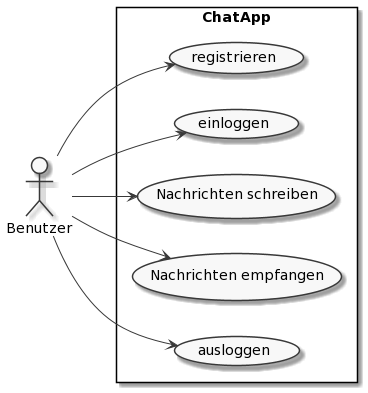
\includegraphics[width=0.6\textwidth]{Graphics/Usecase-Diagramm.png}
	\caption{Use-Case Diagramm}
\end{figure}

\section{Architekturentwurf}

\subsection{Übersicht}
Wie in Abbildung \ref{entwurf} zu sehen ist besteht die Architektur aus einem Client mit graphischer Oberfläche (UI) einem API-Gateway, das alle Anfragen von Clienten empfängt und drei Microservices mit je einer eigenen Datenbank, die die Hauptfunktionalitäten des Systems implementieren.

\subsection{Microservices}
Jede Funktion aus den Anforderungen korrespondiert mit einem Microservice. Die Aufteilung der Microservices ergibt sich aus der Annahme, dass die Funkionalitäten, die sie bereitstellen unterschiedlich oft genutzt werden: Anzahl der Registrierungen < Anzahl Login/Logout < Anzahl der geschriebenen Nachrichten/Abruf von Nachrichten). Daraus gewinnen wir eine individuelle Skalierbarkeit der Funktionen, ohne Redundanz.

\subsection{Registration-Microservice}
Über den Registration-Microservice kann sich ein Benutzer registrieren. Dazu stellt er eine Schnittstelle zur Verfügung an die man eine Nachricht mit E-Mail, Passwort und Land senden kann. Beim Eintreffen einer neuen Nachricht wird ein neuer Eintrag in seiner Datenbank generiert. Des Weiteren wird eine Nachricht an den Login-Service gesendet, mit der Anfrage, auch hier den neuen Benutzer anzulegen.

\subsection{Login-Microservice}
Der Login-Microservice stellt drei verschiedene Funktionen über eine Schnittstelle zur Verfügung: Anlegen eines neuen Benutzers, Einloggen und Ausloggen. Soll ein neuer Benutzer angelegt werden (dies wird vom Registration-Microservice angestoßen), so erzeugt der Microservice einen neuen Eintrag in der Login-Datenbank, in dem E-Mail (auch als ID verwendet) und Passwort des Benutzers gespeichert werden. Will sich ein Benutzer anmelden, gleicht der Microservice die Daten mit der Datenbank ab und stellt dem Benutzer, falls die Kredentialen korrekt waren, einen Token aus, welcher auch in der Datenbank gespeichert wird. Mit diesem Token, kann er sich dann bei anderen Microservices dann authorisieren. Meldet sich ein Benutzer ab, wird der Token einfach aus der Datenbank gelöscht.

\subsection{Message-Microservice}
Die Schnittstelle des Message-Microservices umfasst das Senden einer Nachricht und das Abrufen von empfangenen Nachrichten. Im Fall des Sendens müssen die folgenden Daten angegeben werden: eine Nachricht, eine empfänger E-Mail Adresse und einen Token. Mithilfe des Tokens stellt der Message-Microservice sicher, dass der Sender eine gültige Session hat. Dazu sendet er eine entsprechende Nachricht an den Login-Microservice, der dann den Token bestätigt oder ablehnt. Im positiven Fall wird die Nachricht in der Datenbank des Microservices gespeichert. Will ein Benutzer seine Nachrichten abrufen, so muss er nur einen gültigen Token vorzeigen, den der Message-Microservice, wie beim Senden einer Nachricht, über den Login-Microservice abgleicht.

\subsection{API-Gateway}
Das API-Gateway schottet die Microservices ab. Das bedeutet, dass alle Anfragen vom Clienten nur an das API-Gateway gesendet werden und niemals direkt an die Microservices. Das Gateway leitet dann die Anfrage an den entsprechenden Mircoservice weiter und sendet dessen Antwort wieder an den Clienten. Die Abschottung hat mehrere Vorteile. Sicherheitsrelevante Aspekte wie z.B. DDOS-Protection oder der Schutz vor unbefugtem Zugriff (von Adressen, die nicht zum Client gehören) können auf das API-Gateway verlagert werden und müssen daher nicht in jedem Microservice implementiert werden.
Des Weiteren erfüllt das API-Gateway die Rolle eines Load-Balancers, der die Anfragen auf verschiedene Instanzen von Microservices verteilt. 

\subsection{Client}
Mithilfe des Clients können Anfragen an das System, genauer gesagt das API-Gateway, gesendet werden. Er enthält keine Funktionalitäten und dient lediglich zum Abrufen und Darstellen von Inhalten.

\begin{figure}[bth] 
	\centering
	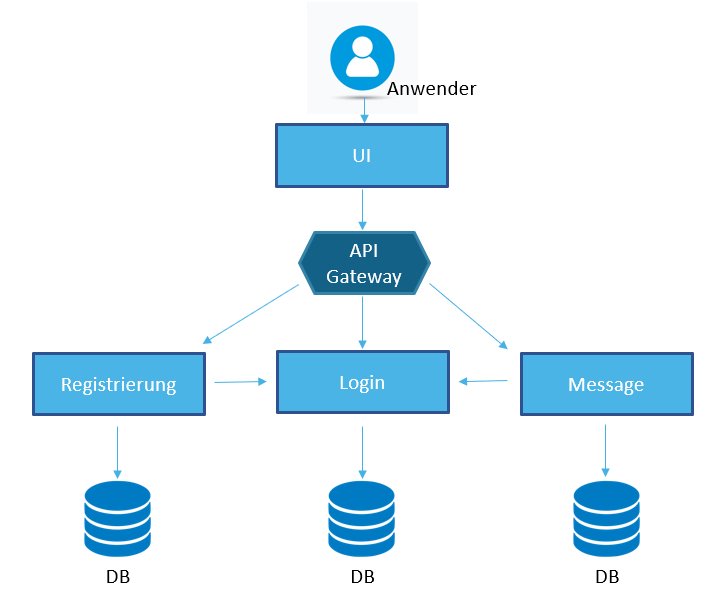
\includegraphics[width=0.6\textwidth]{Graphics/Architekturentwurf.png}
	\caption{Architekturentwurf}
	\label{entwurf}
\end{figure}

\begin{figure}[bth] 
	\centering
	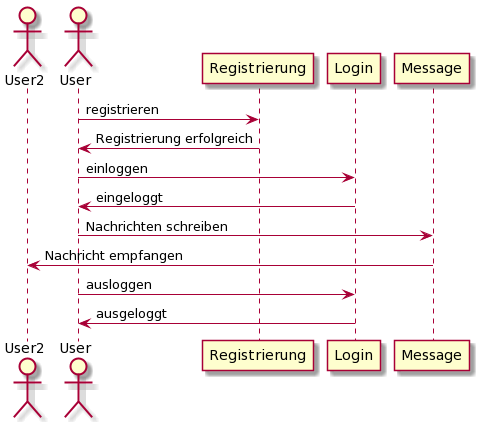
\includegraphics[width=0.6\textwidth]{Graphics/Sequenzdiagramm.png}
	\caption{Sequenzdiagramm}
\end{figure}

\section{Implementierung des Prototyps}

In diesem Kapitel stellen wir unsere prototypische Implementierug vor. Das gesamte System ist in fünf Teile aufgeteilt (UI, API-Gateway, Registration-Microservice, Login-Microservice und Message-Microservice), wobei jeder Teil einem unabhängigem Projekt entspricht, aus welchem jeweils ein eigenständig ausführbares Programm ensteht.
Sämtliche Kommunikation wird über das HTTP Protokoll abgewickelt. Die Inhalte der Nachrichten sind dabei im JSON Format.

\subsection{UI}
TODO


\subsection{API-Gateway}
Das API-Gateway ist mit Java und Maven als Build-Management-Tool implementiert. Es stellt eine HTTP Schnittstelle zur Verfügung, an die Nachrichten gesendet werden können, die es dann an die Microservices weiterleitet. Für das Gateway sind die Microservices ebenfalls über HTTP Schnittstellen erreichbar.
Das Loadbalancing ist für den Message-Microservice implementiert. Dabei kennt das API-Gateway zwei verschiedene Endpunkte unter denen jeweils eine Instanz des Message-Microservices auf Anfragen hört. Bekommt das Gateway eine Anfrage für den Message-Microservice wird abwechselnd eine der beiden Instanzen ausgewählt, an welche die Anfrage weitergeleitet wird. Die Wahl von zwei Instanzen ist hier zwecks Einfachheit gewählt. Es ist möglich mehr als nur zwei Instanzen des Message-Microservices oder eines anderen Microservices zu verwenden. Eine Möglichkeit um die Lastenverteiltung zu Regeln wäre das Round-Robin-Verfahren, bei dem die Anfragen der Reihe nach auf die Microservices verteilt werden.

\subsection{Microservices}
Alle Microservices sind mit Java und Maven als Build-Management-Tool implementiert. Die Wahl der Programmiersprache und anderen Tools ist könnte dabei beliebig gewählt sein. Entscheidend ist nur die Schnittstelle die nach außen hin zur Verfügung stellt wird. Des Weiteren sind die Microservices Zustandslos. Für den Registration-Microservice und den Message-Microservice ist dies trivial, da sie sowieso keine temporären Daten speichern müssen. Der Login-Microservice muss sich jedoch den Token merken, den jeder Benutzer zur Authorisierung verwendet. Dies tut er indem er den Token in der Datenbank speichert.
Der Einfach halber wurden die Datenbanken für den Registration-Microservice und den Login-Microservice mit einfachen Java Klassen implementiert. Dies war aber für den Message-Microservice nicht möglich, da für ihn immer mindestens zwei Instanzen existieren, welche dann getrennte Daten hätten. Um zumindest die Lösungsidee zu demonstrieren, haben wir eine einfache Datei als Datenbank verwenden, die für beide Instanzen immer zugänglich ist.
%\cleardoublepage\include{Chapters/KapitelBachelorarbeit} % <<< Hier alle Chapter der Abschlussarbeit (einzeln) einbinden

%********************************************************************
% Bibliography/References
%*******************************************************
\cleardoublepage%********************************************************************
% Bibliography
%*******************************************************
\printbibliography

%********************************************************************
% List of Figures etc.
%*******************************************************
\cleardoublepage%*******************************************************
% Verzeichnisse (Abbildungen, Tabellen, Listings, etc.)
%*******************************************************
\cleardoublepage
\begingroup
	\let\clearpage\relax
	\let\cleardoublepage\relax
	\listoffigures
	\listoftables
	%\addcontentsline{toc}{chapter}{\lstlistlistingname}
	\lstlistoflistings 
\endgroup 
%*******************************************************
% Abkürzungsverzeichnis
%*******************************************************
\chapter*{Abkürzungsverzeichnis}
\addcontentsline{toc}{chapter}{Abkürzungsverzeichnis}	
	%Hier alle benötigten Abkürzungen einfügen
	\begin{acronym}[WLAN] % LONGEST ACRONYM HERE FOR CORRECT SPACING
	    \acro{JSON}{JavaScript Object Notation}
	    \acro{API}{Application Programming Interface}
	\end{acronym}
	
	

% ********************************************************************
% Appendix/Anhang
%***************************************************************
\appendix
\part*{Anhang}
\cleardoublepage%********************************************************************
% Appendix
%*******************************************************
\chapter{Erster Abschnitt des Anhangs}
In den Anhang gehören "`Hintergrundinformationen"', also weiterführende Information, ausführliche Listings, Graphen, Diagramme oder Tabellen, die den Haupttext mit detaillierten Informationen ergänzen. 

\blindtext
\blindtext
\blindtext



%*******************************************************
\cleardoublepage\pagestyle{empty}

\hfill

\vfill


\pdfbookmark[0]{Kolophon}{colophon}
\section*{Kolophon}
Dieses Dokument wurde mit der \LaTeX-Vorlage für Abschlussarbeiten an der htw saar im Bereich Informatik/Mechatronik-Sensortechnik erstellt (\currentVersion). Die Vorlage wurde von Yves Hary und Andr\'e Miede entwickelt (mit freundlicher Unterstützung von Thomas Kretschmer, Helmut G. Folz und Martina Lehser). Daten: (F)\makeatletter\f@size\makeatother\ -- (B)\the\textwidth\ -- (H)\the\textheight\ 


\end{document}
% ********************************************************************
